\chapter{Introducción}
\label{cap:Introduccion}
Con todo lo expuesto antes, se puede concluir en que este trabajo se centrará en la creación de un \textbf{sistema inteligente} para la gestión de energía en el hogar de la manera más óptima y eficiente posible. En función de un escenario determinado en una hora t (situación meteorológica, precio del kilovatio-hora (kwh) en el mercado eléctrico, nivel de carga de las baterías de almacenaje, etc) se modelará la cantidad de energía eléctrica recibida por cada una de las entradas. De igual modo, se modelará la cantidad de energía eléctrica suministrada a cada una de las salidas. Esto se traduce en una optimización y aprovechamiento de la energía, que además tiene como consecuencia un ahorro económico en la obtención de la energía necesaria.
En la Figura~\ref{fig:abstract} se muestra un esquema del sistema donde se identifican desde un alto nivel de abstracción las entradas y salidas.\\

\begin{figure}[!h]
	\centering
	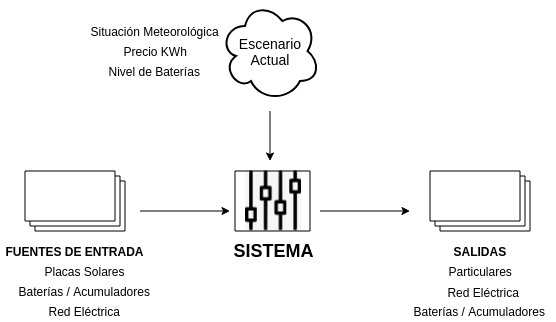
\includegraphics[width=10cm]{figs/Abstract.png}
	\caption{Dibujo del sistema}
        \label{fig:abstract}
\end{figure}
